\documentclass[8pt,a4paper,compress]{beamer}

\usepackage{/home/siyer/lib/slides}

\title{Type Checking}
\date{}

\begin{document}
\begin{frame}
\vfill
\titlepage
\end{frame}

\begin{frame}
\frametitle{Outline}
\tableofcontents
\end{frame}

\section{Introduction}
\begin{frame}[fragile]
\pause

Type checking (aka semantic analysis) is the final step in the analysis phase, and includes the following

\begin{itemize}
\item Determining the types of all names and expressions.
\item Insuring that all expressions are properly typed, for example that the operands of an operator have the proper types
\item A certain amount of storage analysis, for example determining the amount of storage that is required in the current stack frame to store a local variable (one word for \lstinline{int}s, two words for \lstinline{long}s); this information is used to allocate locations (at offsets from the base of the current stack frame) for parameters and local variables
\item A certain amount of AST tree rewriting, usually to make implicit constructs more explicit
\end{itemize}
\end{frame}

\begin{frame}[fragile]
\pause

Semantic analysis of \jmm programs involves all of these operations
\begin{itemize}
\item Like Java, \jmm is strictly-typed, ie, we want to determine the types of all names and expressions at compile time
\item A \jmm program must be well-typed, ie, the operands to all operations must have appropriate types
\item All \jmm local variables (including formal parameters)  must be allocated storage and assigned locations within a method's stack frame
\item The AST for \jmm requires a certain amount of sub-tree rewriting; for example, field references using simple names must be rewritten as explicit field selection operations, and declared variable initializations must be rewritten as explicit assignment statements
\end{itemize}
\end{frame}

\section{The \protect\jmm Types}
\begin{frame}[fragile]
\pause

A type in \jmm is either a primitive type or a reference type

\pause
\bigskip

\jmm primitive types
\begin{itemize}
\item \lstinline{int} - 32 bit two's complement integers
\item \lstinline{boolean} - taking the value \lstinline{true} or \lstinline{false}
\item \lstinline{char} - 16 bit Unicode (but many systems deal only with the lower 8 bits)
\end{itemize}

\pause
\bigskip

\jmm reference types
\begin{itemize}
\item arrays
\item objects of a type described by a class declaration
\item built-in objects \lstinline{java.lang.Object} and \lstinline{java.lang.String}
\end{itemize}

\pause
\bigskip

\jmm code may interact with classes from the Java library but it must be able to do so using only these types
\end{frame}

\begin{frame}[fragile]
\pause

How do we represent the types \lstinline{int}, \lstinline{int[]}, \lstinline{Factorial}, \lstinline{String[][]}?  

\pause
\bigskip

We want a simple, but extensible representation; we want no more complexity than is necessary for representing all of the types in \jmm and for representing any (Java) types that we may add in exercises

\pause
\bigskip

We want the ability to interact with the existing Java class libraries

\pause
\bigskip

Possible solutions
\begin{enumerate}
\item Java types are represented by objects of (Java) type \lstinline{java.lang.Class}; since \jmm is a subset of Java, why not use \lstinline{Class} objects to represent its types? 
\item Define an abstract class (or interface) \lstinline{Type}, and concrete sub-classes (or implementations) \lstinline{PrimitiveType}, \lstinline{ReferenceType}, and \lstinline{ArrayType}
\end{enumerate}
\end{frame}

\begin{frame}[fragile]
\pause

Our solution is to define our own class \lstinline{Type} for representing types, with a simple interface but also encapsulating the \lstinline{java.lang.Class} object that corresponds to the Java representation for that same type

\pause
\bigskip

Since the parser does not know anything about types, we define two placeholder type representations
\begin{enumerate}
\item \lstinline{TypeName} - for representing named types recognized by the parser like user-defined classes or imported classes until such time as they may be resolved to their proper \lstinline{Type} representation
\item \lstinline{ArrayTypeName} - for representing array types recognized by the parser like \lstinline{String[]}, until such time that they may resolved to their proper \lstinline{Type} representation
\end{enumerate}

\pause
\bigskip

During analysis, \lstinline{TypeName}s and \lstinline{ArrayTypeName}s are resolved to the \lstinline{Type}s that they represent

\pause
\bigskip

More specifically
\begin{itemize}
\item A \lstinline{TypeName} is resolved by looking it up in the current context, our symbol table representation, and the \lstinline{Type} found replaces the \lstinline{TypeName}, and finally, the \lstinline{Type}'s accessibility from the place the \lstinline{TypeName} is encountered is checked
\item Since an \lstinline{ArrayTypeName} has a base type, the base type is resolved to a \lstinline{Type}, whose \lstinline{Class} representation becomes the base type for representing the array type
\item A \lstinline{Type} resolves to itself
\end{itemize}
\end{frame}

\section{\protect\jmm Symbol Tables}
\begin{frame}[fragile]
\pause

A symbol table maps names to the things they name, for example, types, formal parameters and local variables; these mappings are established in a declaration and consulted each time a declared name is encountered

\pause
\bigskip

In the \jmm compiler, the symbol table is a tree of \lstinline{Context} objects, which spans the abstract syntax tree, with each \lstinline{Context} corresponding to a region of scope in the \jmm source program

\pause
\bigskip

For example, reconsider the simple \lstinline{Factorial} program.  In this version we mark two locations in the program using comments: \lstinline{position 1} and \lstinline{position 2}

\begin{lstlisting}[language=Java]
package pass;

import java.lang.System;

public class Factorial {
    public static int factorial(int n) {
        // position 1:
        if (n <= 0) {
            return 1;
        } else {
            return n * factorial(n - 1);
        }
    }

    public static void main(String[] args) {
        // position 2:
        int x = n;
        System.out.println(n + "! = " + factorial(x));
    }

    static int n = 5;
}
\end{lstlisting}
\end{frame}

\begin{frame}[fragile]
\pause

The symbol table for the \lstinline{Factorial} program, and its relationship to the AST, is illustrated in figure below

\begin{center}
\visible<2->{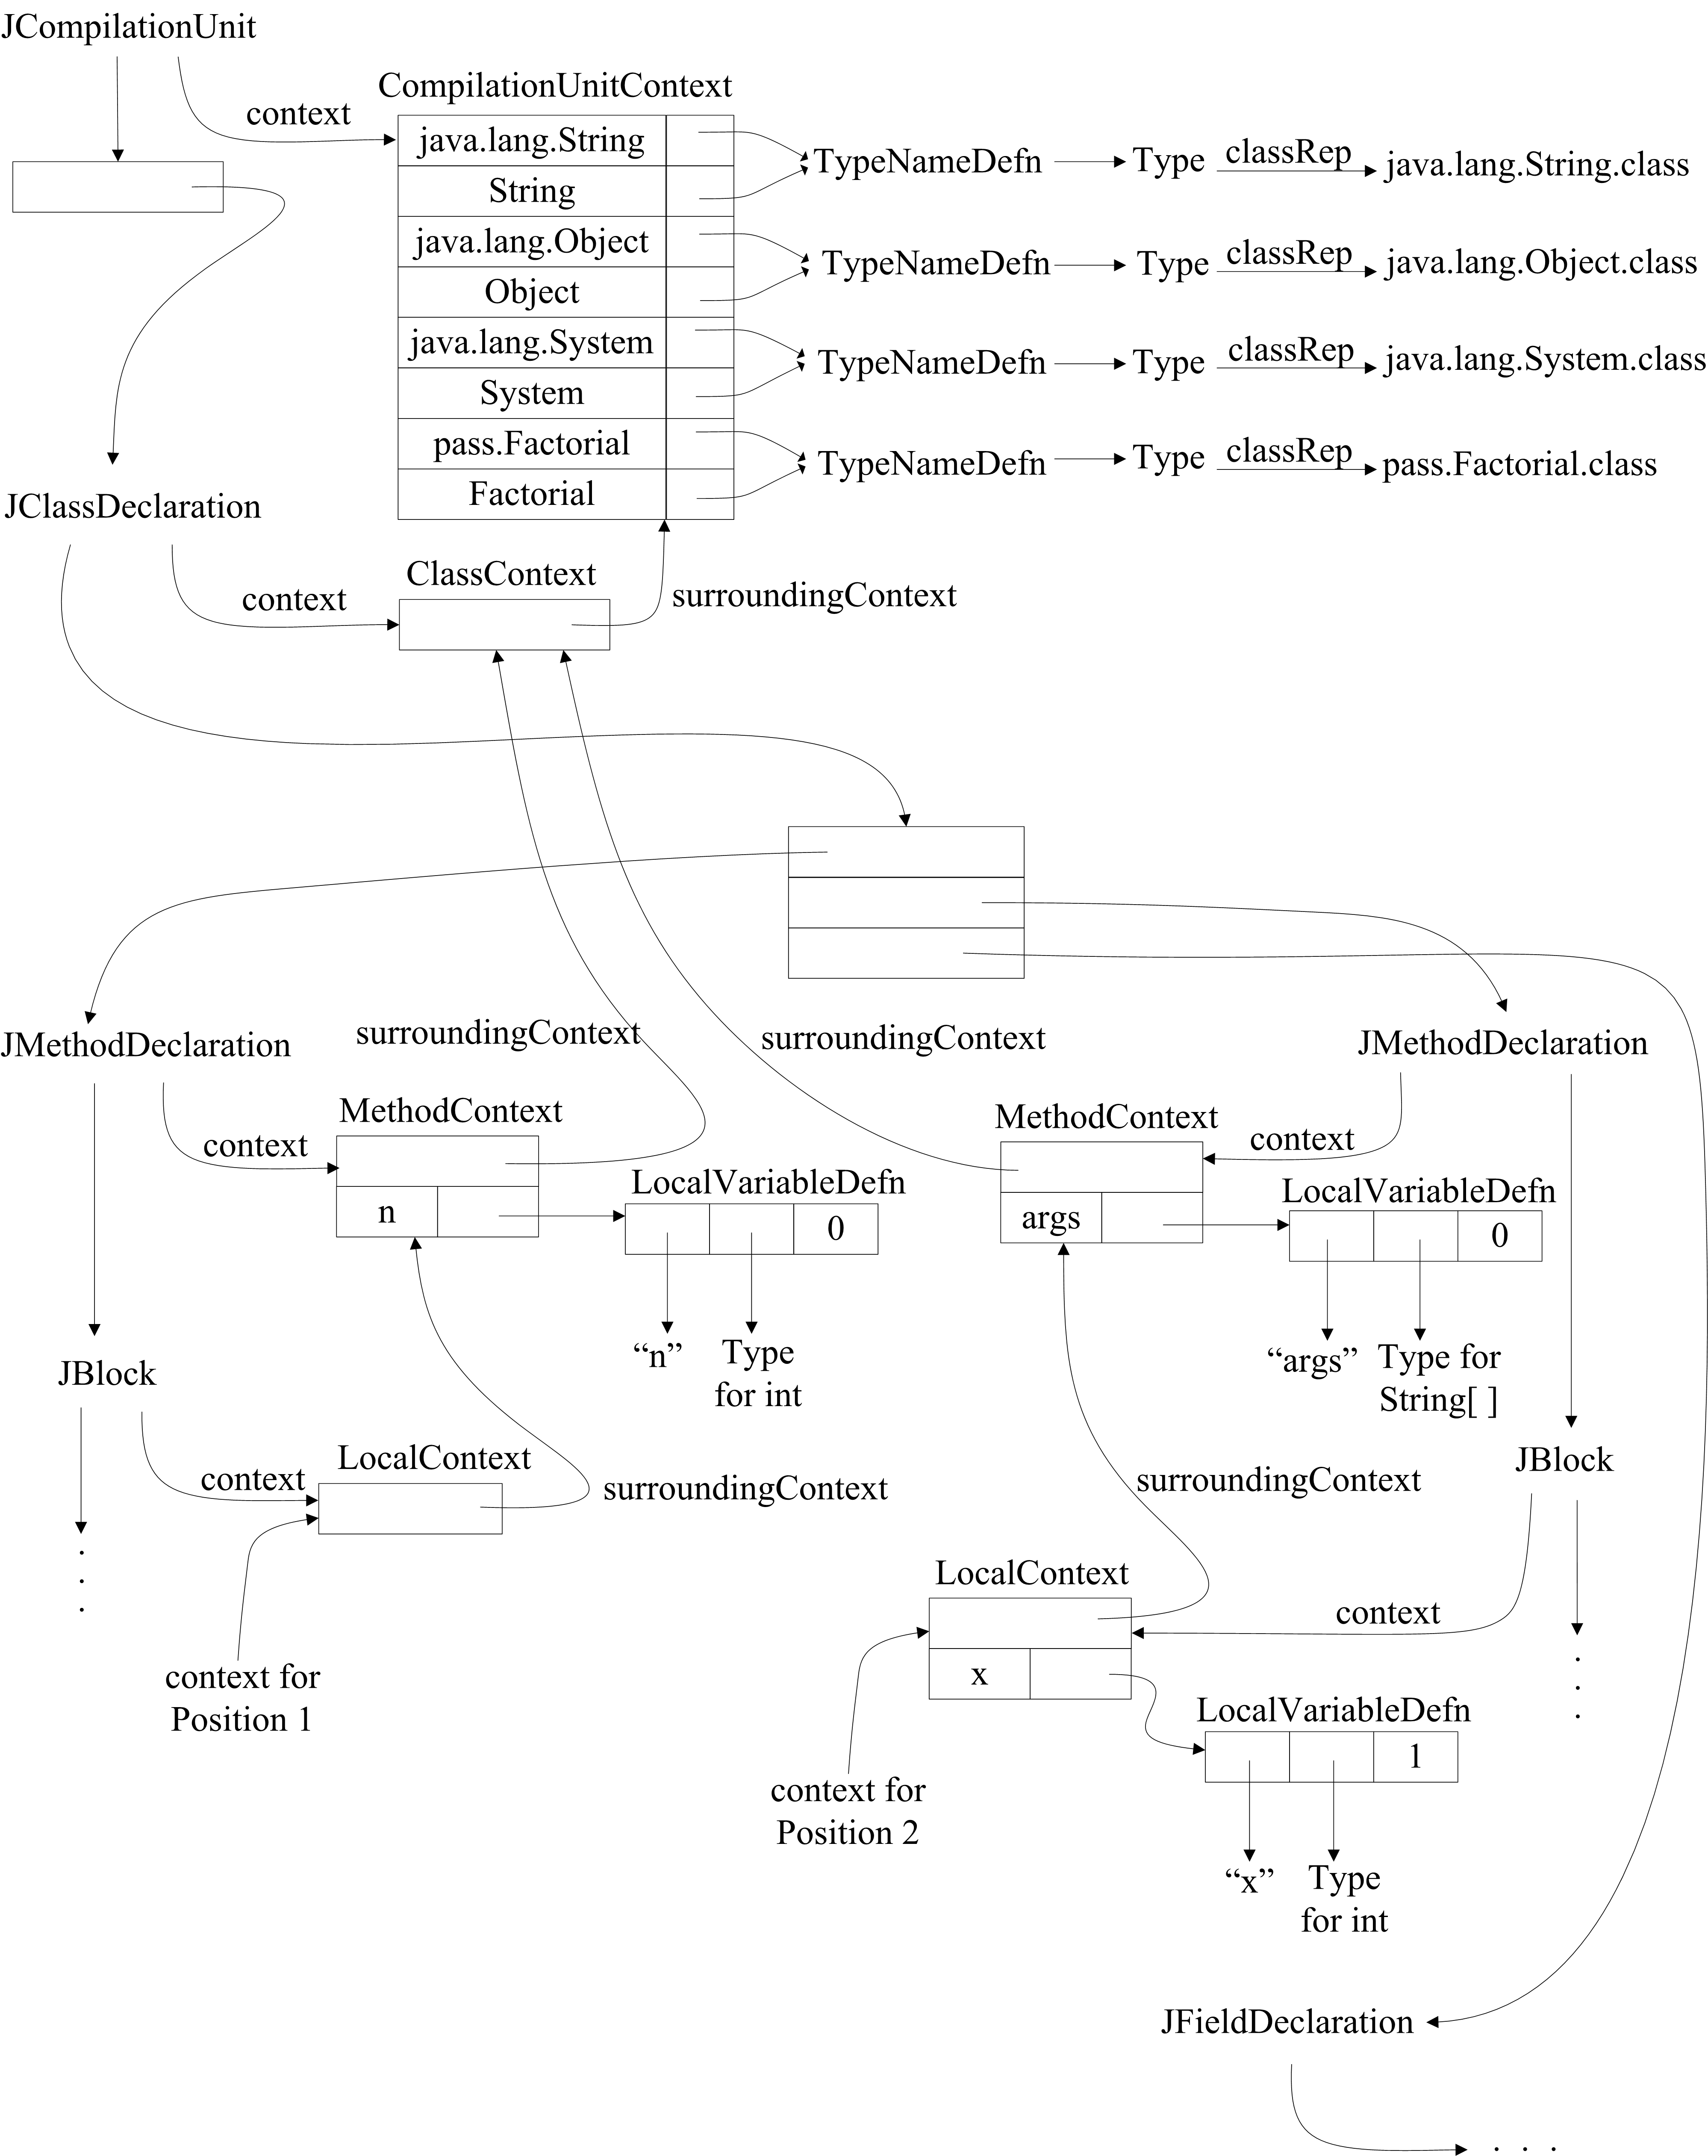
\includegraphics[scale=0.29]{{figures/figure04.01}.jpg}}
\end{center}
\end{frame}

\begin{frame}[fragile]
\pause

The symbol table takes the form of a tree that corresponds to the shape of the AST

\pause
\bigskip

A \lstinline{context}, ie, a node in this tree, captures the region of scope corresponding to the AST node that points to it

\pause
\bigskip

For example, in the above figure
\begin{enumerate}
\item The context pointer from the AST's \lstinline{JCompilationUnit} node points to the \lstinline{JCompilationUnitContext} that is at the root of the symbol table
\item The context pointer from the AST's \lstinline{JClassDeclaration} points to a \lstinline{ClassContext}
\item The context pointer from the AST's two \lstinline{JMethodDeclaration}s each point to a \lstinline{MethodContext}
\item The context pointer from the AST's two \lstinline{JBlock}s each point to a \lstinline{LocalContext}
\end{enumerate}

\pause
\bigskip

From any particular location in the program, looking back towards the root \lstinline{CompilationUnitContext}, the symbol table looks like a stack of contexts

\pause
\bigskip

Each \lstinline{surroundingContext} link back towards the \lstinline{CompilationUnitContext} points to the context representing the surrounding lexical scope
\end{frame}

\begin{frame}[fragile]
\pause

During analysis, when the compiler encounters a variable, it looks up that variable in the symbol table by name, beginning at the \lstinline{LocalContext} most recently created in the symbol table

\pause
\bigskip

Type names are looked up in the \lstinline{CompilationUnitContext}; to facilitate this, each context maintains three pointers to surrounding contexts, as illustrated in the following figure

\begin{center}
\visible<3->{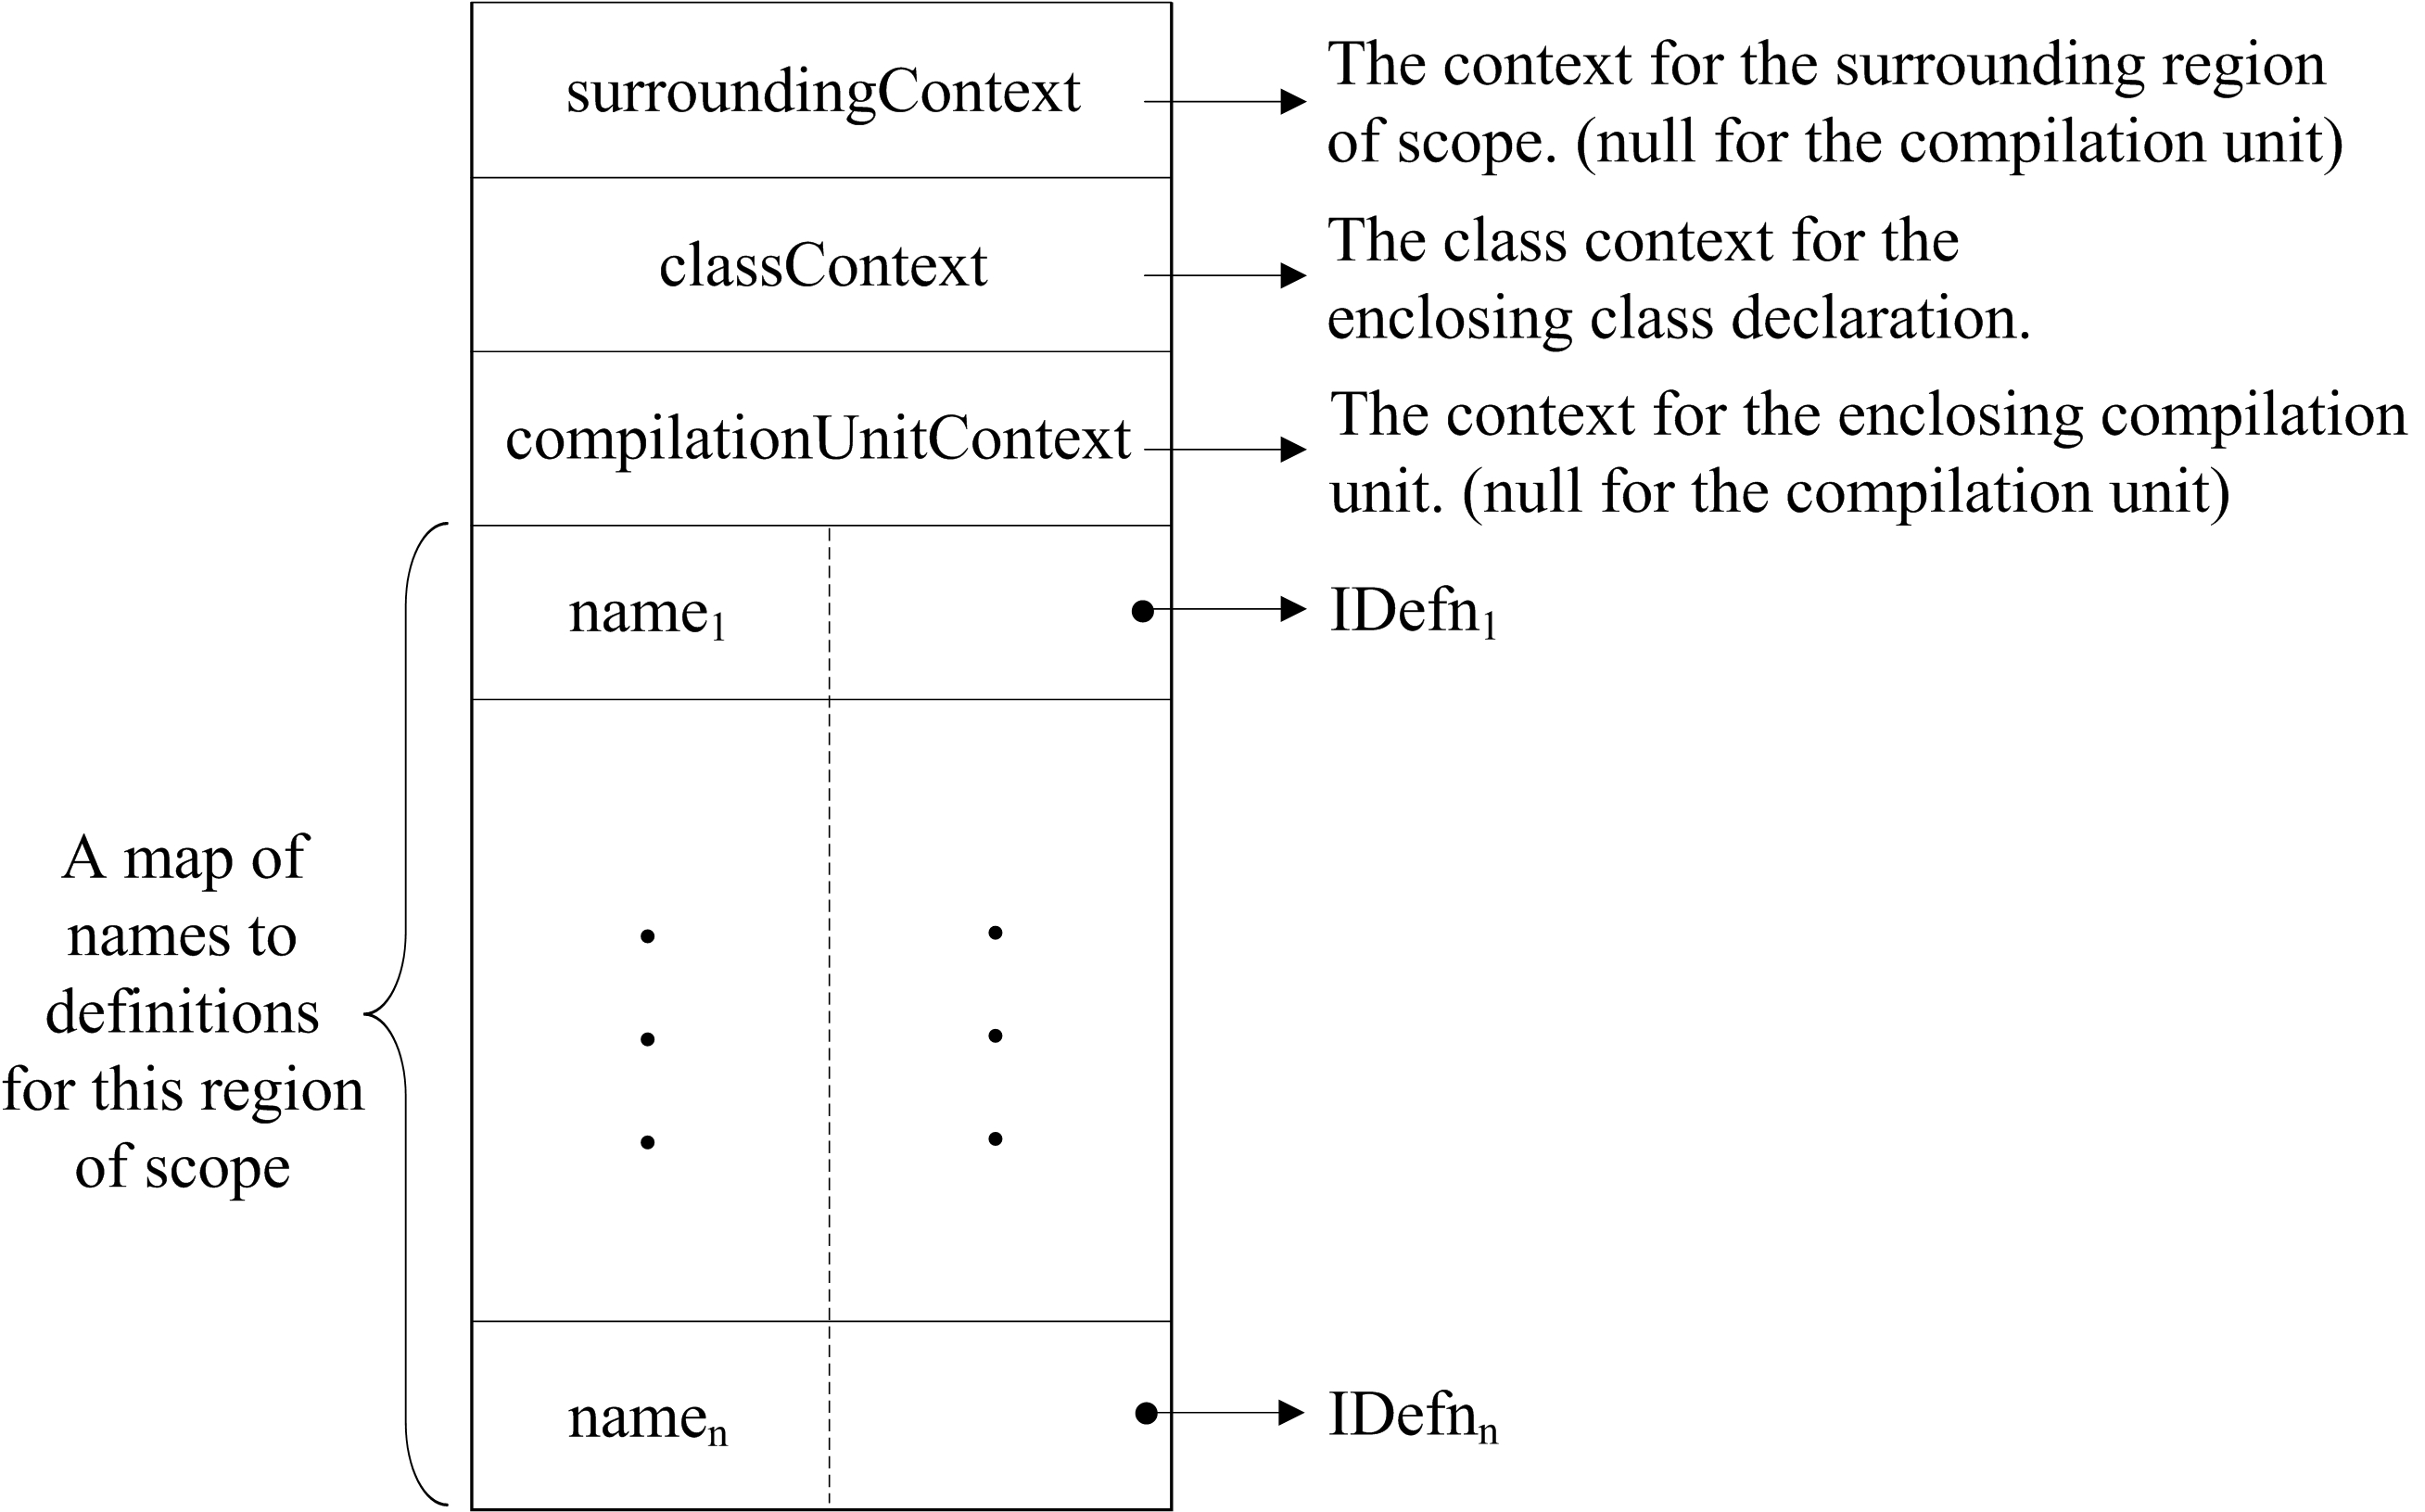
\includegraphics[scale=0.5]{{figures/figure04.02}.jpg}}
\end{center}
\end{frame}

\begin{frame}[fragile]
\pause

A \lstinline{CompilationUnitContext} represents the scope of the entire program and contains a mapping from names to types
\begin{itemize}
\item The implicitly declared types, \lstinline{java.lang.Object}, and \lstinline{java.lang.String}
\item Imported types
\item User-defined types, that is, types introduced in clss declarations
\end{itemize}

\pause
\bigskip

A \lstinline{ClassContext} represents the scope within a class declaration; in the \jmm symbol table, no names are declared here, but if we were to add nested type declarations to \jmm, they might be declared here

\pause
\bigskip

A \lstinline{MethodContext} represents the scope within a method declaration; a method's formal parameters are declared here

\pause
\bigskip

A \lstinline{LocalContext} represents the scope within a block, which includes the block defining the body to a method; local variables are declared here
\end{frame}

\begin{frame}[fragile]
\pause

Each kind of context derives from (extends) the class \lstinline{Context}, which supplies the mapping from names to definitions (\lstinline{IDefns})

\pause
\bigskip

The inheritance tree for contexts is illustrated in the following figure
\begin{center}
\visible<3->{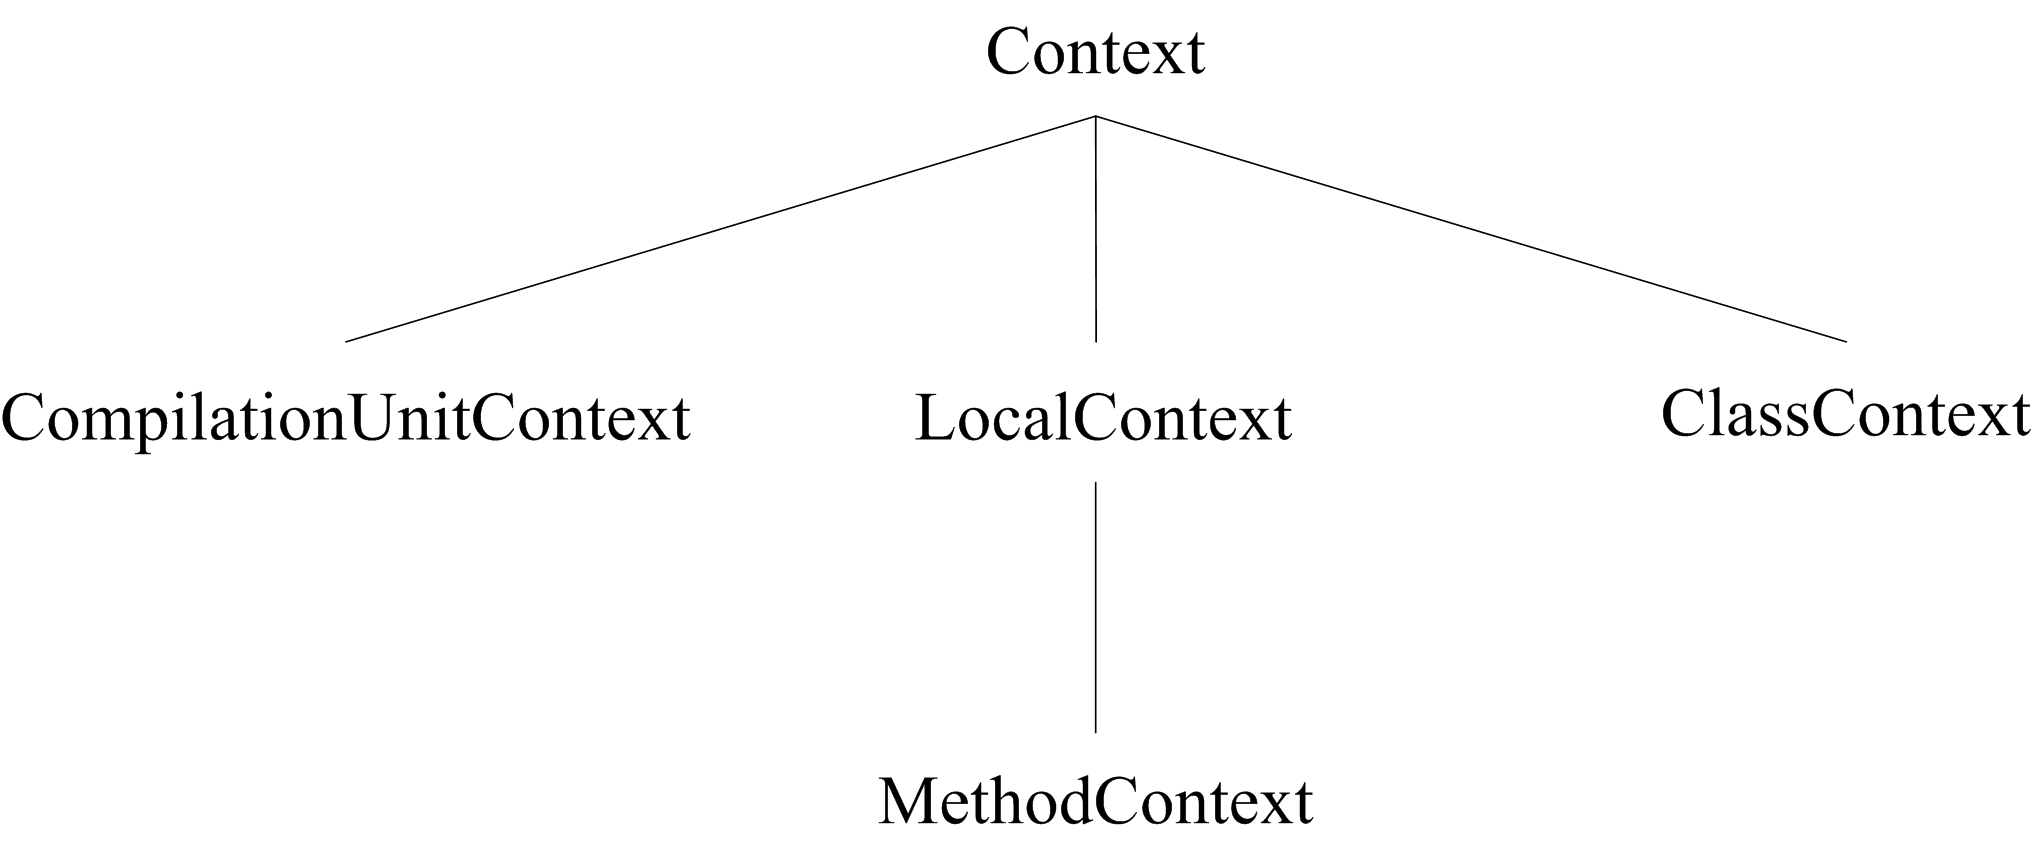
\includegraphics[scale=0.5]{{figures/figure04.03}.jpg}}
\end{center}

\pause
\bigskip

An \lstinline{IDefn} is the interface type for symbol table definitions, which has two implementations
\begin{enumerate}
\item A \lstinline{TypeNameDefn}, which defines a type name; an \lstinline{IDefn} of this sort encapsulates the \lstinline{Type} that it denotes
\item A \lstinline{LocalVariableDefn} defines a local variable and encapsulates the name, its \lstinline{Type} and an offset in the current run-time stack frame
\end{enumerate}
\end{frame}

\begin{frame}[fragile]
\pause

Class member (field and method in \jmm) names are not declared in a \lstinline{ClassContext}, but in the \lstinline{Type}s that they declare

\pause
\bigskip

We rely on the encapsulated \lstinline{Class} object to store the interface information, and we rely on Java reflection to query a type for information about its members

\pause
\bigskip

For example, \lstinline{Type} supports a method \lstinline{fieldFor()} which, when given a name returns a \lstinline{Field} with the given name that is defined for that type

\begin{lstlisting}[language=Java]
public Field fieldFor(String name) {
    Class<?> cls = classRep;
    while (cls != null) {
        java.lang.reflect.Field[] fields = cls.getDeclaredFields();
        for (java.lang.reflect.Field field:fields) {
            if (field.getName().equals(name)) {
                return new Field(field);
            }
        }
        cls = cls.getSuperclass();
    }
    return null;
}
\end{lstlisting}
\end{frame}

\section{Pre-analysis of \protect\jmm Programs}
\begin{frame}[fragile]
\pause

The semantic analysis of \jmm  programs requires two traversals of the AST because a class name or a member name may be referenced before it is declared in the source program

\pause
\bigskip

The traversals are accomplished by the method \lstinline{preAnalyze()} for the first traversal and the method \lstinline{analyze()} for the second, which invoke themselves at the child nodes for recursively descending the AST

\pause
\bigskip

The \lstinline{preAnalyze()} method must traverse down the AST only far enough for
\begin{itemize}
\item Declaring imported type names
\item Declaring user-defined class names
\item Declaring fields
\item Declaring methods (including their signatures - the types of their parameters)
\end{itemize}

\pause
\bigskip

Therefore, \lstinline{preAnalyze()}need be defined only in the following types of AST nodes
\begin{itemize}
\item \lstinline{JCompilationUnit}
\item \lstinline{JClassDeclaration}
\item \lstinline{JFieldDeclaration}
\item \lstinline{JMethodDeclaration}
\item \lstinline{JConstructorDeclaration}
\end{itemize}
\end{frame}

\begin{frame}[fragile]
\pause

For the \lstinline{JCompilationUnit} node at the top of the AST, \lstinline{preAnalyze()} does the following
\begin{enumerate}
\item It creates a \lstinline{CompilationUnitContext}
\item It declares the implicit \jmm types, \lstinline{java.lang.String} and \lstinline{java.lang.Object}
\item It declares any imported types
\item It declares the types defined by class declaration, ie, creates a \lstinline{Type} for each declared class, whose \lstinline{classRep} refers to a \lstinline{Class} object for an empty class; for example, in the pre-analysis phase of our \lstinline{Factorial} program above, the \lstinline{Type} for \lstinline{Factorial} would have a \lstinline{classRep}, the \lstinline{Class} object for the class
\begin{lstlisting}[language=Java]
class Factorial {}
\end{lstlisting}
\item Finally, \lstinline{preAnalyze()} invokes itself for each of the type declarations in the compilation unit
\end{enumerate}

\pause
\bigskip

Here is the code for \lstinline{preAnalyze()} in \lstinline{JCompilationUnit}
\begin{lstlisting}[language=Java]
public void preAnalyze() {
    context = new CompilationUnitContext();

    // Declare the two implicit types java.lang.Object and
    // java.lang.String
    context.addType(0, Type.OBJECT);
    context.addType(0, Type.STRING);
\end{lstlisting}
\end{frame}

\begin{frame}[fragile]
\pause

Here is the code for \lstinline{preAnalyze()} in \lstinline{JCompilationUnit}
\begin{lstlisting}[language=Java]

    // Declare any imported types
    for (TypeName imported: imports) {
        try {
            Class<?> classRep =
                Class.forName(imported.toString());
            context.addType(imported.line(),
                Type.typeFor(classRep));
        }
        catch (Exception e) {
            JAST.compilationUnit.reportSemanticError(
                imported.line(),
                "Unable to find %s", imported.toString());                      
        }
    }

    // Declare the locally declared type(s)
    CLEmitter.initializeByteClassLoader();
    for (JAST typeDeclaration: typeDeclarations) {
        ((JTypeDecl)
              typeDeclaration).declareThisType(context);
    }

    // Pre-analyze the locally declared type(s). Generate
    // (partial) Class instances, reflecting only the member
    // interface type information
    CLEmitter.initializeByteClassLoader();
    for (JAST typeDeclaration: typeDeclarations) {
        ((JTypeDecl)
          typeDeclaration).preAnalyze(context);
    }
}
\end{lstlisting}
\end{frame}

\begin{frame}[fragile]
\pause

In a class declaration, \lstinline{preAnalyze()} does the following
\begin{enumerate}
\item It firstly creates a new \lstinline{ClassContext}, whose \lstinline{surroundingContext} points to the \lstinline{CompilationUnitContext}
\item It resolves the class's super type
\item It creates a new \lstinline{CLEmitter} instance, which will eventually be converted to the \lstinline{Class} object for representing the declared class
\item It adds a class header, defining a name and any modifiers, to this \lstinline{CLEmitter} instance
\item It recursively invokes \lstinline{preAnalyze()} on each of the class's members, which causes field declarations, constructors and method declarations (but with empty bodies) to be added to the \lstinline{CLEmitter} instance
\item If there is no explicit constructor (having no arguments) in the set of members, it adds the implicit constructor to the \lstinline{CLEmitter} instance; for example, for the \lstinline{Factorial} program above, the following implicit constructor is added
\begin{lstlisting}[language=Java]
public Factorial() {
    super();
}
\end{lstlisting}
\item Finally, the \lstinline{CLEmitter} instance produces a \lstinline{Class} object, and that replaces the \lstinline{classRep} for the \lstinline{Type} of the declared class name in the (parent) \lstinline{ClassContext}
\end{enumerate}
\end{frame}

\begin{frame}[fragile]
\pause

Here is the code for \lstinline{preAnalyze()} in \lstinline{JClassDeclaration}
\begin{lstlisting}[language=Java]
public void preAnalyze(Context context) {
    // Construct a class context
    this.context = new ClassContext(this, context);

    // Resolve superclass
    superType = superType.resolve(this.context);

    // Creating a partial class in memory can result in a
    // java.lang.VerifyError if the semantics below are
    // violated, so we can't defer these checks to analyze()
    thisType.checkAccess(line, superType);
    if (superType.isFinal()) {
        JAST.compilationUnit.reportSemanticError(line,
            "Cannot extend a final type: %s",                                   
            superType.toString());
    }

    // Create the (partial) class
    CLEmitter partial = new CLEmitter();

    // Add the class header to the partial class
    String qualifiedName =
        JAST.compilationUnit.packageName() == "" ? name :
            JAST.compilationUnit.packageName() + "/" + name;
    partial.addClass(mods, qualifiedName, superType.jvmName(),
        null, false);
\end{lstlisting}
\end{frame}

\begin{frame}[fragile]
\pause

\begin{lstlisting}[language=Java]

    // Pre-analyze the members and add them to the partial class
    for (JMember member: classBlock) {
        member.preAnalyze(this.context, partial);
        if (member instanceof JConstructorDeclaration &&
             ((JConstructorDeclaration) member).
                 params.size() == 0) {
            hasExplicitConstructor = true;
        }
    }

    // Add the implicit empty constructor?
    if (!hasExplicitConstructor) {
        codegenPartialImplicitConstructor(partial);
    }

    // Get the Class rep for the (partial) class and make it the
    // representation for this type
    Type id = this.context.lookupType(name);
    if (id != null &&
         !JAST.compilationUnit.errorHasOccurred()) {
        id.setClassRep(partial.toClass());
    }
}
\end{lstlisting}

\pause
\bigskip

Here is the code for \lstinline{preAnalyze()} in \lstinline{JMethodDeclaration}
\begin{lstlisting}[language=Java]
public void preAnalyze(Context context, CLEmitter partial) {
    // Resolve types of the formal parameters
    for (JFormalParameter param: params) {
        param.setType(param.type().resolve(context));
    }
\end{lstlisting}
\end{frame}

\begin{frame}[fragile]
\pause

\begin{lstlisting}[language=Java]

    // Resolve return type
    returnType = returnType.resolve(context);

    // Check proper local use of abstract
    if (isAbstract && body != null) {
        JAST.compilationUnit.reportSemanticError(line(),
            "abstract method cannot have a body");
    }
    else if (body == null && ! isAbstract) {
        JAST.compilationUnit.reportSemanticError(line(),
            "Method with null body must be abstract");
    }
    else if (isAbstract && isPrivate ) {
        JAST.compilationUnit.reportSemanticError(line(),
            "private method cannot be declared abstract");
    }
    else if (isAbstract && isStatic ) {
        JAST.compilationUnit.reportSemanticError(line(),
            "static method cannot be declared abstract");
    }

    // Compute descriptor
    descriptor = "(";
    for (JFormalParameter param: params) {
        descriptor += param.type().toDescriptor();
    }
    descriptor += ")" + returnType.toDescriptor();

    // Generate the method with an empty body (for now)
    partialCodegen(context, partial);
}
\end{lstlisting}
\end{frame}

\begin{frame}[fragile]
\pause

The code for \lstinline{partialCodegen()} is as follows
\begin{lstlisting}[language=Java]
public void partialCodegen(Context context, CLEmitter partial) {
    // Generate a method with an empty body; need a return to
    // make the class verifier happy.
    partial.addMethod(mods, name, descriptor, null, false);

    // Add implicit RETURN
    if (returnType == Type.VOID) {
	partial.addNoArgInstruction(RETURN);
    }
    else if (returnType == Type.INT ||
              returnType == Type.BOOLEAN ||
              returnType == Type.CHAR) {
        partial.addNoArgInstruction(ICONST_0);
        partial.addNoArgInstruction(IRETURN);
    }
    else {
        // A reference type.
        partial.addNoArgInstruction(ACONST_NULL);
        partial.addNoArgInstruction(ARETURN);
    }
}
\end{lstlisting}
\end{frame}

\begin{frame}[fragile]
\pause

Pre-analysis for a \lstinline{JFieldDeclaration} is similar to that for a \lstinline{JMethodDeclaration}, and does the following
\begin{enumerate}
\item Enforces the rule that fields may not be declared \lstinline{abstract}
\item Resolves the field's declared type
\item Generates the JVM code for the field declaration, via the \lstinline{CLEmitter} created for the enclosing class declaration
\end{enumerate}

\pause
\bigskip

The code itself is rather simple
\begin{lstlisting}[language=Java]
public void preAnalyze(Context context, CLEmitter partial) {
    // Fields may not be declared abstract.
    if (mods.contains("abstract")) {
        JAST.compilationUnit.reportSemanticError(line(),
            "Field cannot be declared abstract");
    }

    for (JVariableDeclarator decl: decls) {
        // Add field to (partial) class
        decl.setType(decl.type().resolve( context));
        partial.addField(mods, decl.name(),
            decl.type().toDescriptor(), false);
    }
}
\end{lstlisting}
\end{frame}

\begin{frame}[fragile]
\pause

The following figure illustrates how much of the symbol table is constructed for our \lstinline{Factorial} program once pre-analysis is complete

\begin{center}
\visible<2->{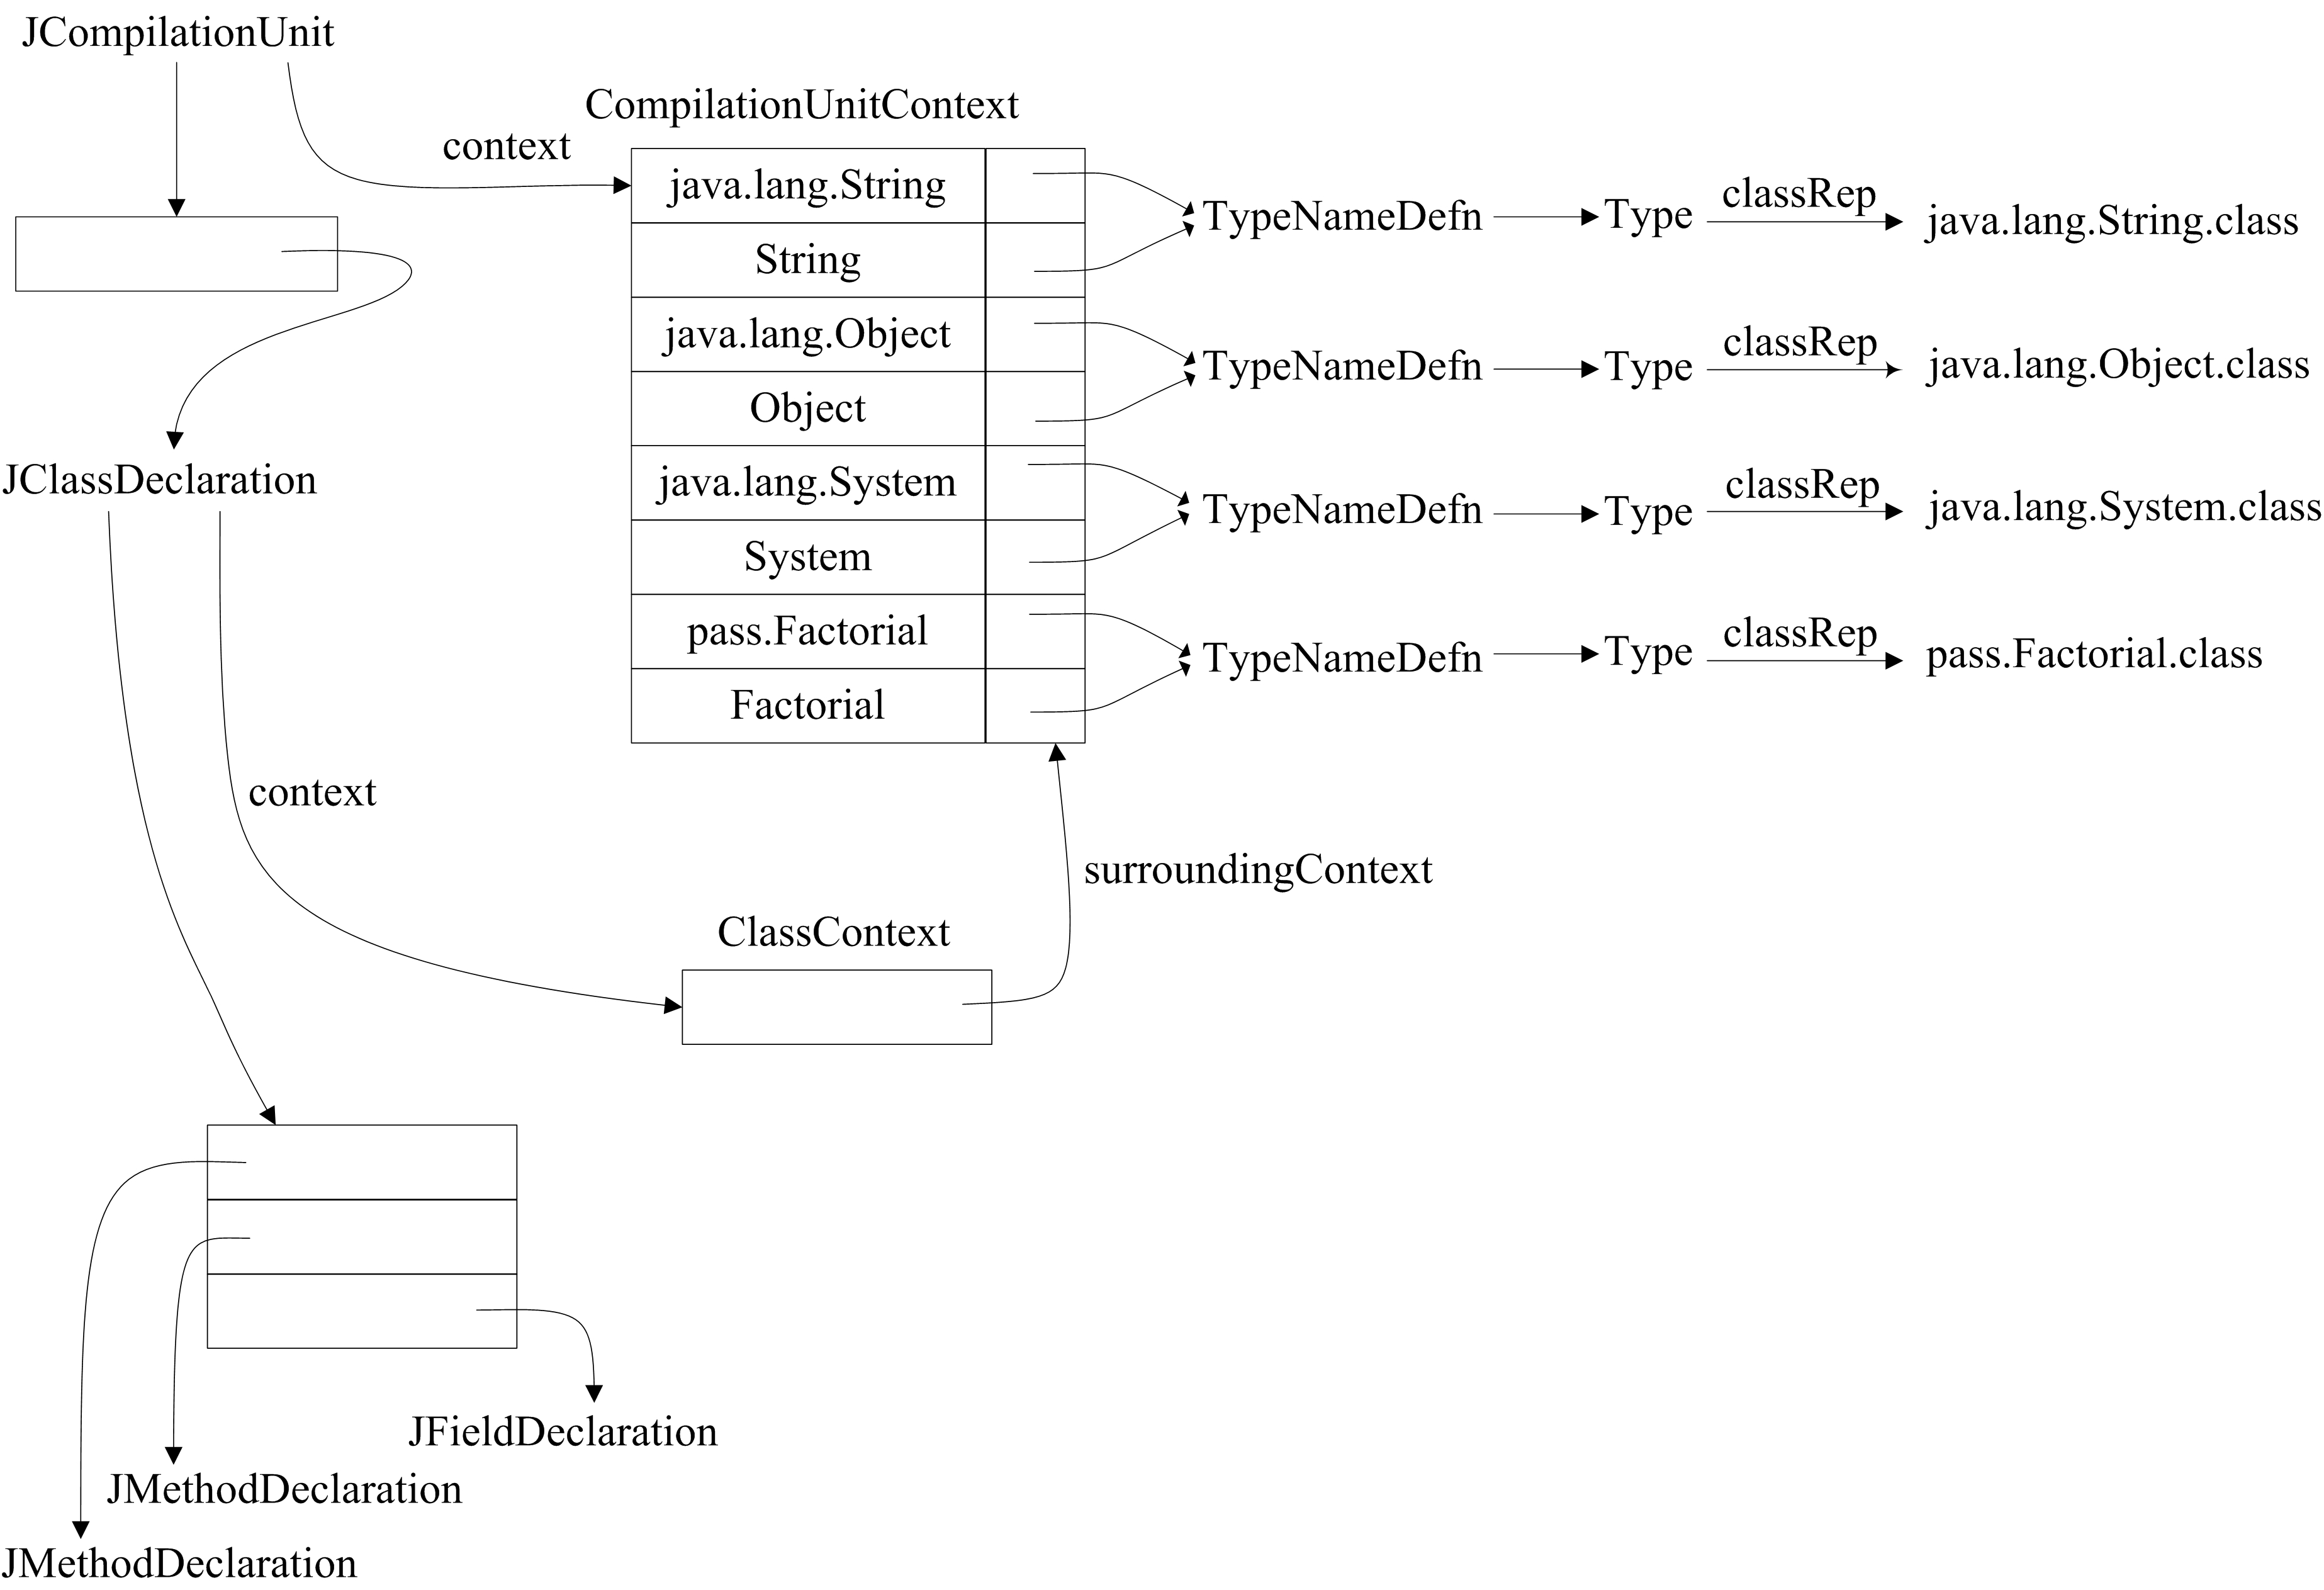
\includegraphics[scale=0.5]{{figures/figure04.04}.jpg}}
\end{center}
\end{frame}

\section{Analysis of \protect\jmm Programs}
\begin{frame}[fragile]
\pause

The analysis phase, ie, the \lstinline{analyze()} method, recursively descends throughout the AST all the way to its leaves
\begin{itemize}
\item Re-writing field and local variable initializations as assignments
\item Declaring both formal parameters and local variables
\item Allocating locations in the stack frame for the formal parameters and local variables
\item Computing the types of expressions and enforcing the language type rules
\item Reclassifying ambiguous names
\item Doing a limited amount of tree surgery
\end{itemize}

\pause
\bigskip

At the top of the AST, \lstinline{analyze()} simply recursively descends into each of the  type (class) declarations, delegating analysis to one class declaration at a time
\begin{lstlisting}[language=Java]
public JAST analyze(Context context) {
    for (JAST typeDeclaration : typeDeclarations) {
        typeDeclaration.analyze(this.context);
    }
    return this;
}
\end{lstlisting}
\end{frame}

\begin{frame}[fragile]
\pause

In \lstinline{JFieldDeclaration}, \lstinline{analyze()} rewrites the field initializer as an explicit assignment statement, analyzes that and then stores it in the \lstinline{JFieldDeclaration}'s initializations list
\begin{lstlisting}[language=Java]
public JFieldDeclaration analyze(Context context) {
    for (JVariableDeclarator decl : decls) {
        // All initializations must be turned into assignment
        // statements and analyzed
        if (decl.initializer() != null) {
            JAssignOp assignOp = new JAssignOp(decl.line(), 
                                     new JVariable(decl.line(), 
                                         decl.name()), decl.initializer());
            assignOp.isStatementExpression = true;
            initializations.add(new JStatementExpression(decl.line(), 
                                assignOp).analyze(context));
        }
    }
    return this;
}
\end{lstlisting}

\pause
\bigskip

In \lstinline{JClassDeclaration}, \lstinline{analyze()} separates the assignment statements into two lists: one for the static fields and one for the instance fields
\begin{lstlisting}[language=Java]
// Copy declared fields for purposes of initialization.
for (JMember member : classBlock) {
    if (member instanceof JFieldDeclaration) {
        JFieldDeclaration fieldDecl = (JFieldDeclaration) member;
        if (fieldDecl.mods().contains("static")) {
            staticFieldInitializations.add(fieldDecl);
        } else {
            instanceFieldInitializations.add(fieldDecl);
        }
    }
}
\end{lstlisting}
\end{frame}

\begin{frame}[fragile]
\pause

The following figure shows how the static field declaration (\lstinline{static int n = 5;}) in the \lstinline{Factorial} program is rewritten
\begin{center}
\visible<2->{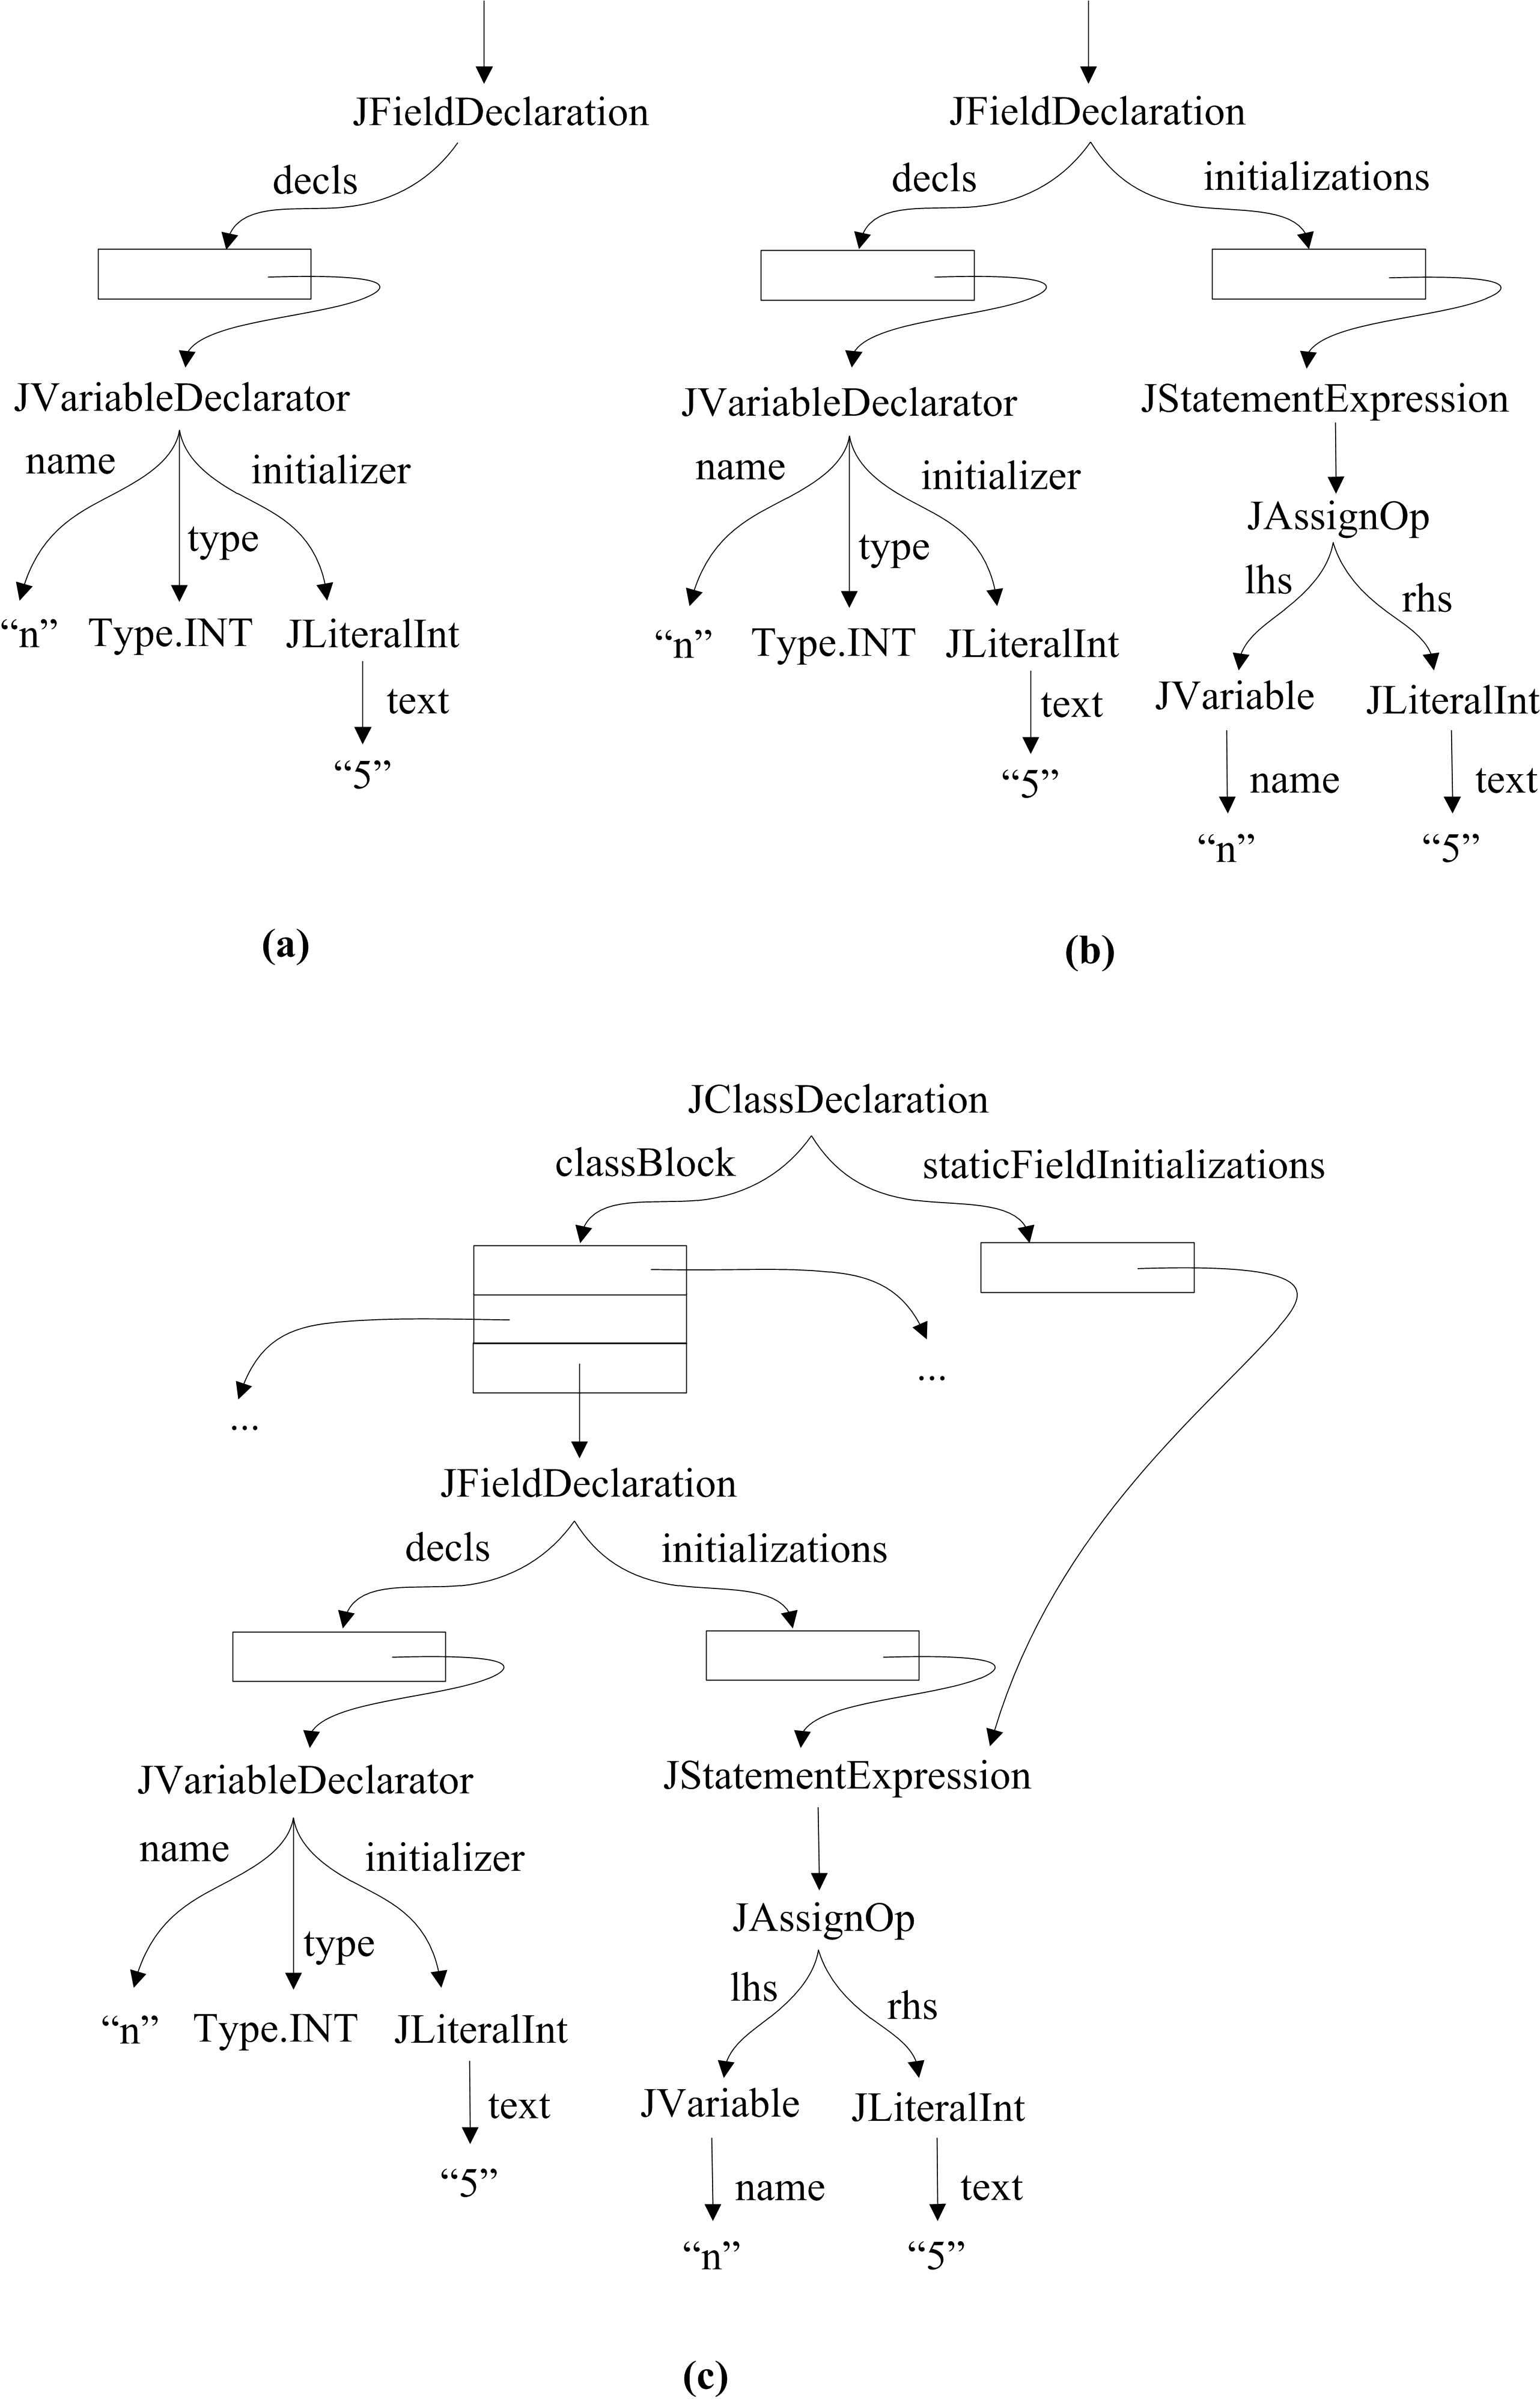
\includegraphics[scale=0.35]{{figures/figure04.05}.jpg}}
\end{center}
\end{frame}

\begin{frame}[fragile]
\pause

Both formal parameters and local variables are declared in the symbol table and allocated locations within a method invocation's run-time stack frame

\pause
\bigskip

For example, consider the following class declaration
\begin{lstlisting}[language=Java]
public class Locals {
    public int foo(int t, String u) {
        int v = u.length();
        {
            int w = v + 5, x = w + 7;
            v = w + x;
        }
        {
            int y = 3;
            int z = v + y;
            t = t + y + z;
        }
        return t + v;
    }
}
\end{lstlisting}
\end{frame}

\begin{frame}[fragile]
\pause

The stack frame allocated for an invocation of \lstinline{foo()} at run time by the JVM is shown below
\begin{center}
\visible<2->{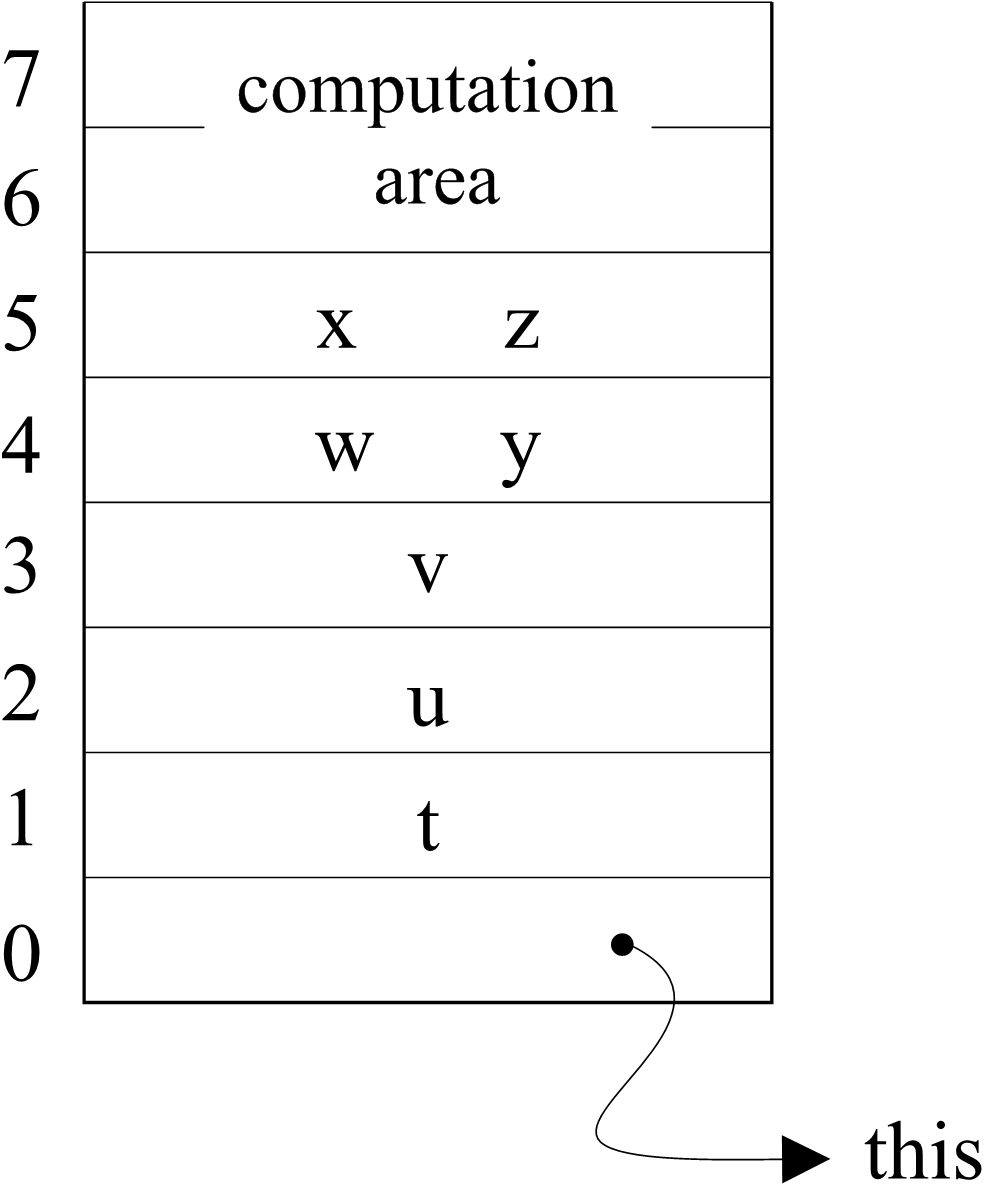
\includegraphics[scale=0.5]{{figures/figure04.06}.jpg}}
\end{center}

\pause
\bigskip

The code for analyzing a \lstinline{JMethodDeclaration} performs four steps
\begin{enumerate}
\item It creates a new \lstinline{MethodContext}, whose \lstinline{surroundingContext} points back to the previous \lstinline{ClassContext}
\item The first stack frame offset is 0; but if this is an instance method then offset 0 must be allocated to \lstinline{this}, and the \lstinline{nextOffset} is incremented to 1
\item The formal parameters are declared as local variables and allocated consecutive offsets in the stack frame
\item It analyzes the method's body
\end{enumerate}
\end{frame}

\begin{frame}[fragile]
\pause

\begin{lstlisting}[language=Java]
public JAST analyze(Context context) {
    this.context = new MethodContext(context, returnType);

    if (!isStatic) {
        // Offset 0 is used to addr "this".
        this.context.nextOffset();
    }

    // Declare the parameters
    for (JFormalParameter param : params) {
        this.context.addEntry(param.line(), param.name(),
                new LocalVariableDefn(param.type(), this.context
                        .nextOffset(), null));
    }

    if (body != null) {
        body = body.analyze(this.context);
    }
    return this;
}
\end{lstlisting}
\end{frame}

\begin{frame}[fragile]
\pause

The code for analyzing a \lstinline{JBlock} performs two steps
\begin{enumerate}
\item It creates a new \lstinline{LocalContext}, whose \lstinline{surroundingContext} points back to the previous \lstinline{MethodContext} (or \lstinline{LocalContext} in the case of nested blocks); its \lstinline{nextOffset} value is copied from the previous context
\item It analyzes each of the body's statements; any \lstinline{JVariableDeclaration}s declare their variables in the \lstinline{LocalContext} created in step 1; any nested \lstinline{JBlock} simply invokes this two-step process recursively, creating yet another \lstinline{LocalContext} for the nested block
\end{enumerate}

\pause
\bigskip

\begin{lstlisting}[language=Java]
public JBlock analyze(Context context) {
    // { ... } defines a new level of scope.
    this.context = new LocalContext(context);

    for (int i = 0; i < statements.size(); i++) {
        statements.set(i, (JStatement) statements.get(i).analyze(
                this.context));
    }
    return this;
}
\end{lstlisting}
\end{frame}

\begin{frame}[fragile]
\pause

The stages of the symbol table in analyzing \lstinline{Locals.foo()}
\begin{center}
\visible<2->{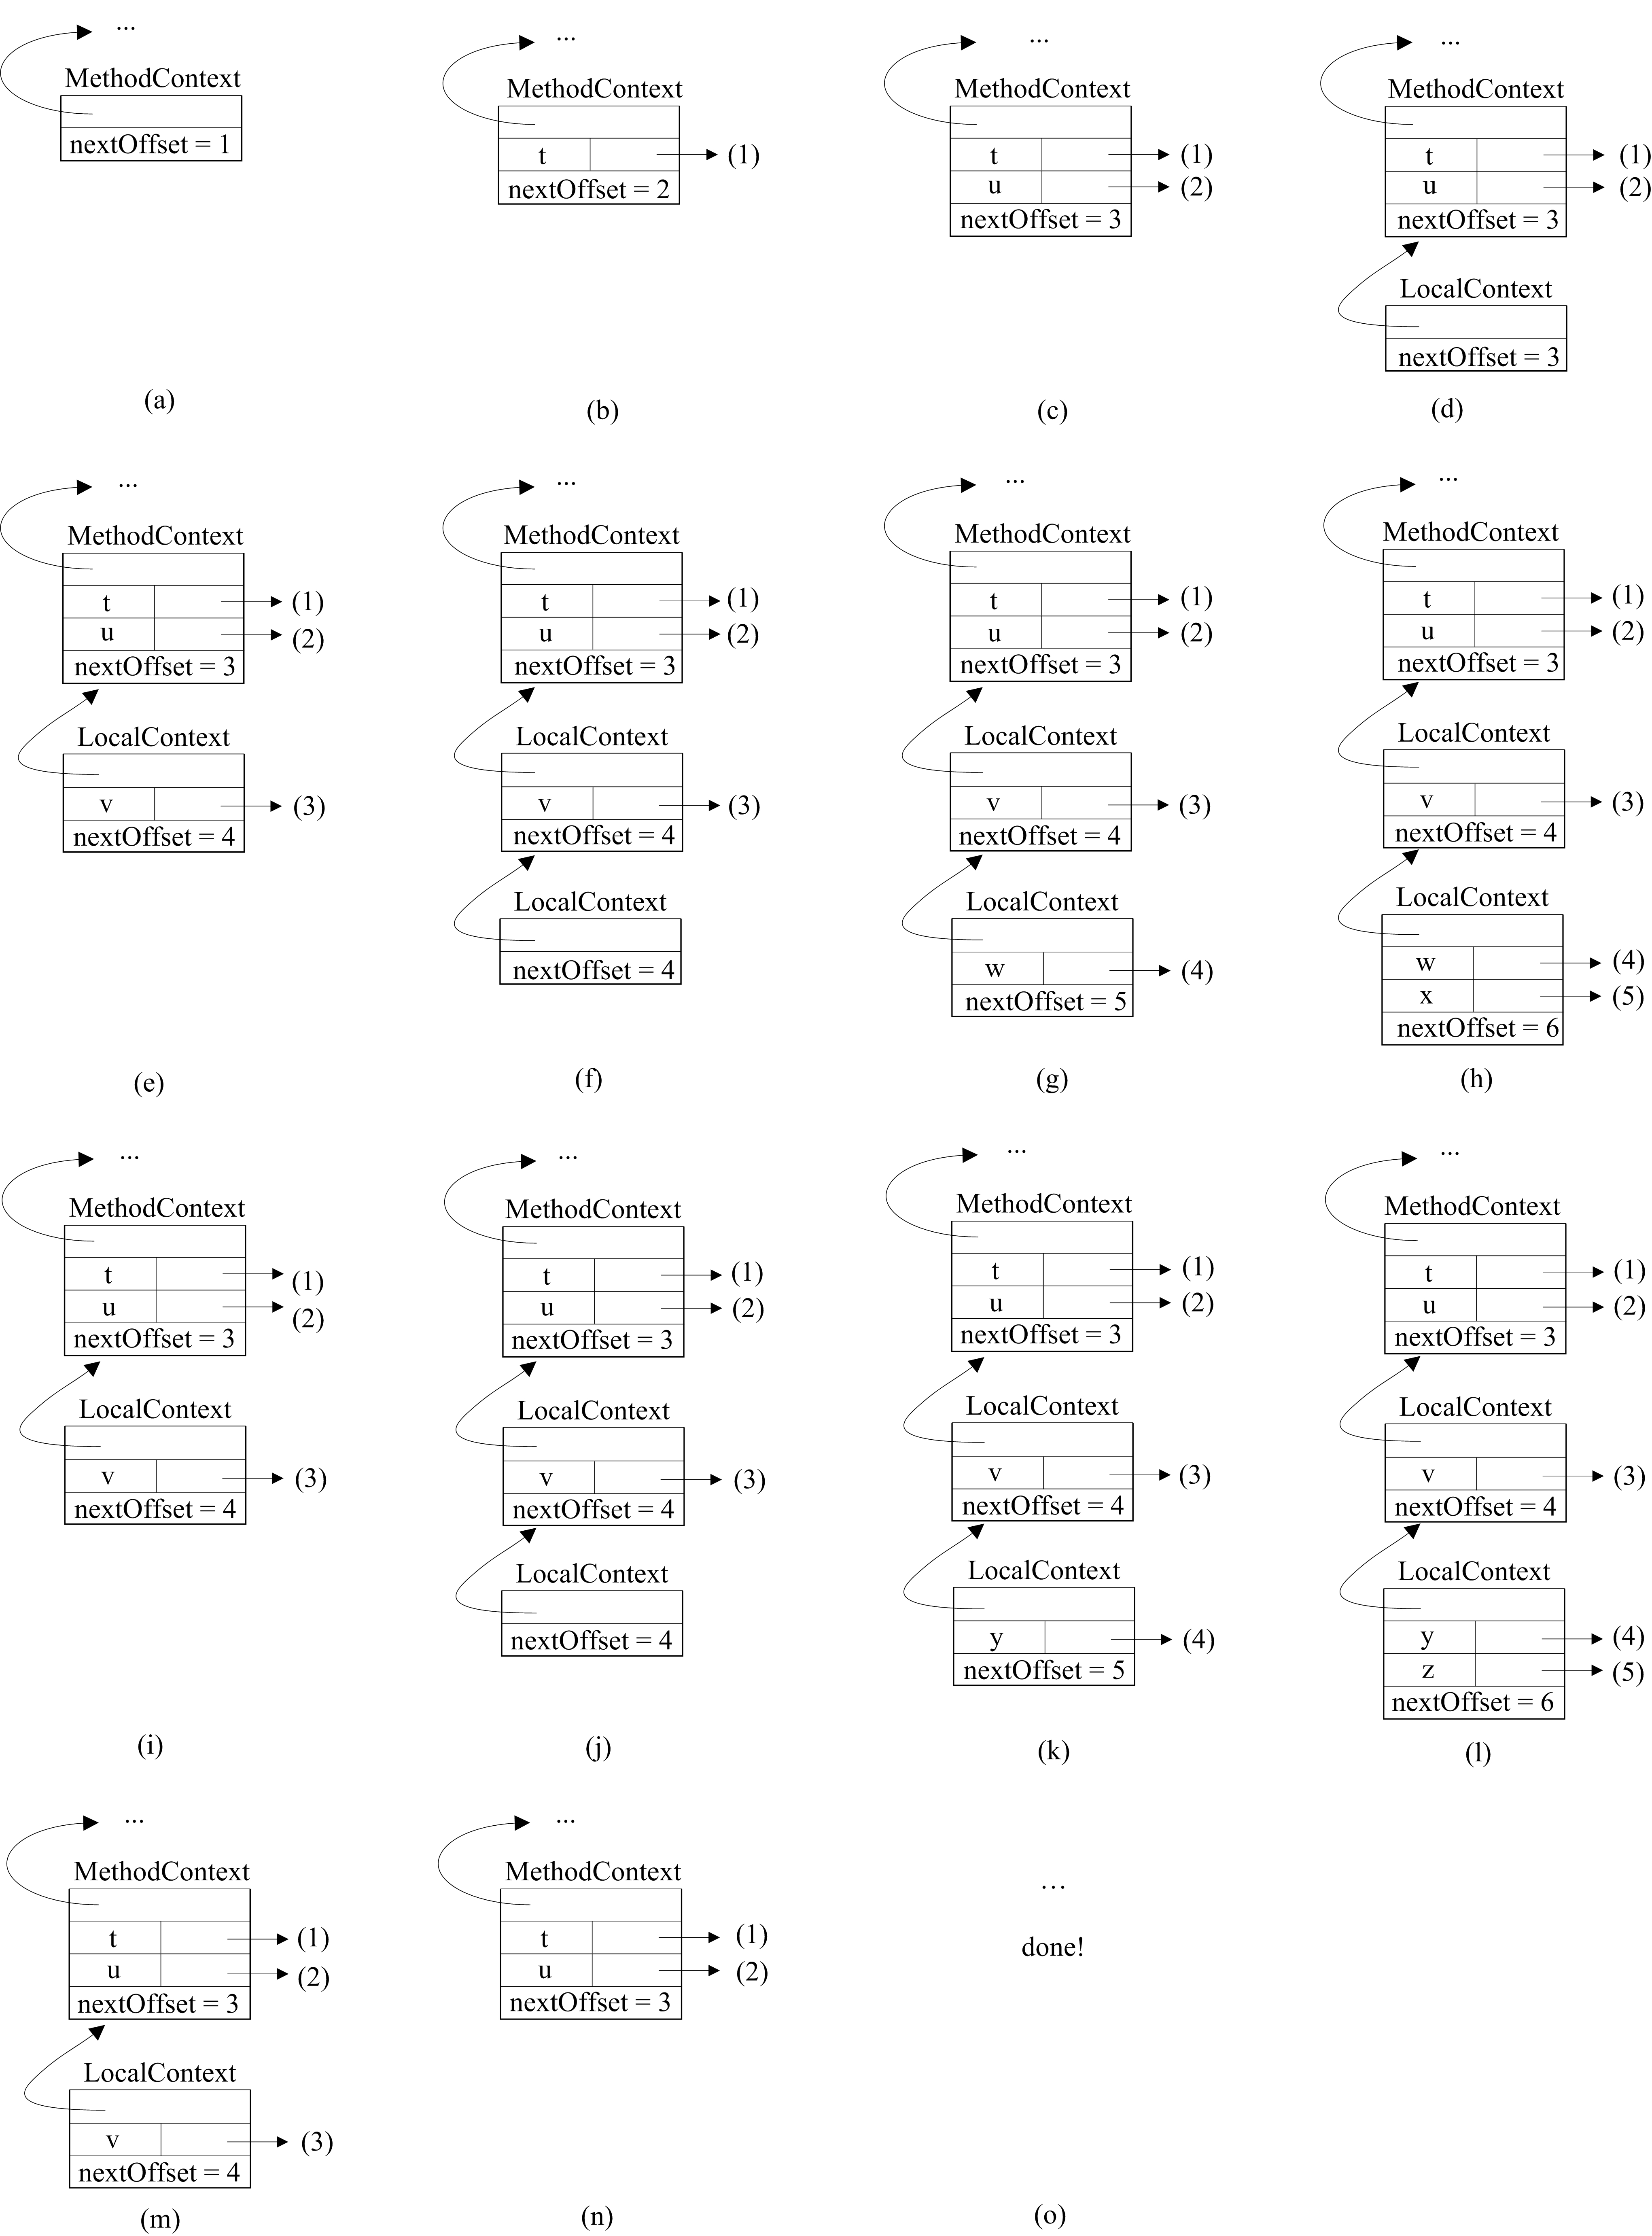
\includegraphics[scale=0.3]{{figures/figure04.07}.jpg}}
\end{center}
\end{frame}

\begin{frame}[fragile]
\pause


\end{frame}

\begin{frame}[fragile]
\pause


\end{frame}

\begin{frame}[fragile]
\pause


\end{frame}

\begin{frame}[fragile]
\pause


\end{frame}
\end{document}
